\begin{figure*}
    \centering
    \begin{subfigure}{\textwidth}
        \centering
        \begin{minipage}[c]{0.05\textwidth}
            \rotatebox{90}{\textbf{All pretext tasks}}
        \end{minipage}
        \begin{minipage}[c]{0.7\textwidth}
            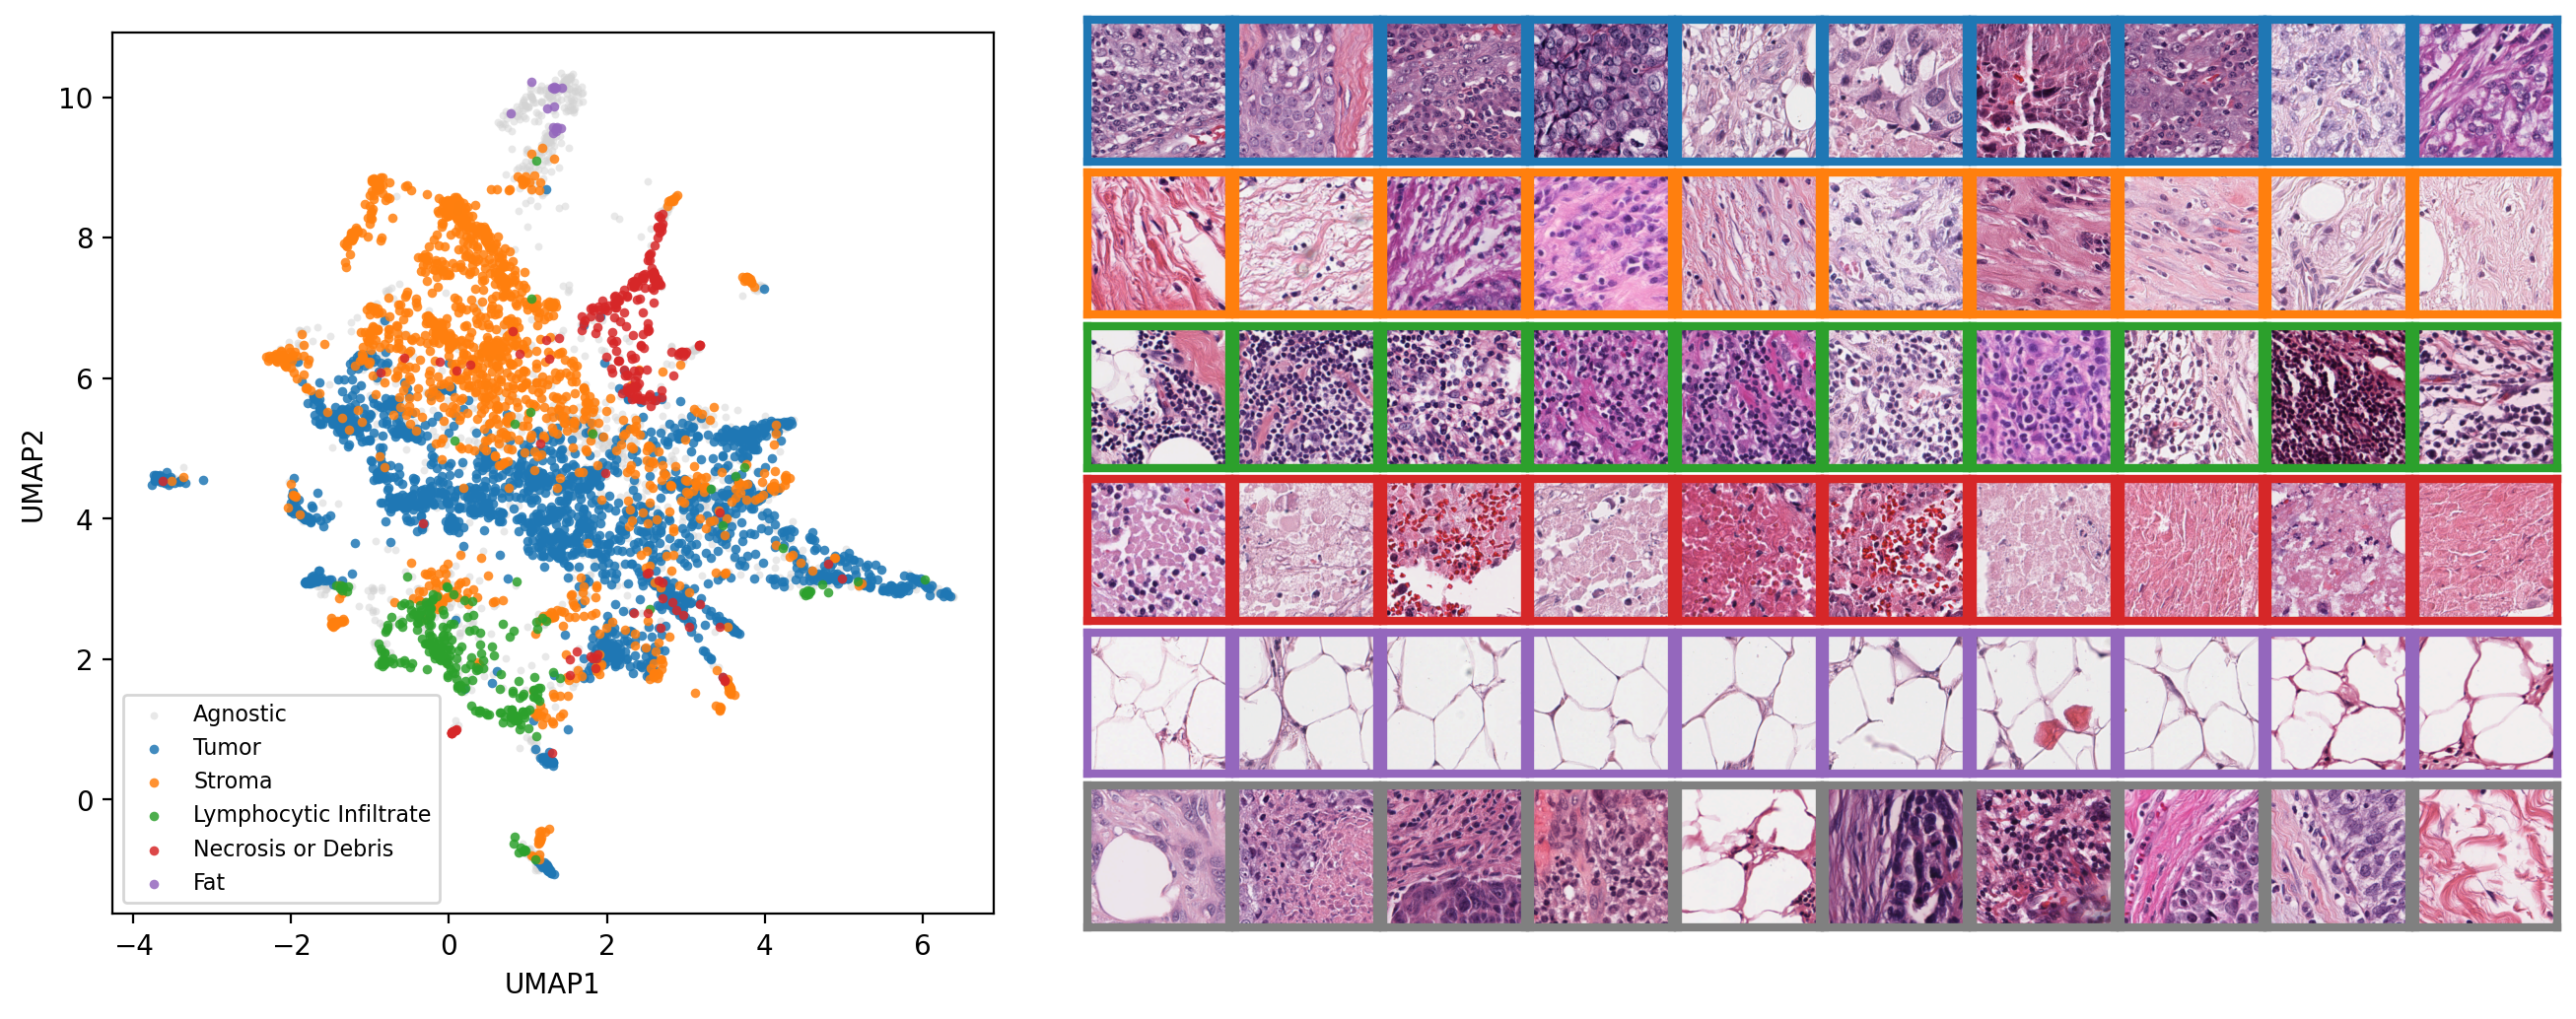
\includegraphics[width=1.0\linewidth]{images/resnet50-full_umap_encoder_model-prediction_top-5.png}
        \end{minipage}
    \end{subfigure}
    \begin{subfigure}{\textwidth}
        \centering
        \begin{minipage}[c]{0.05\textwidth}
            \rotatebox{90}{\textbf{Hematoxylin}}
        \end{minipage}
        \begin{minipage}[c]{0.7\textwidth}
            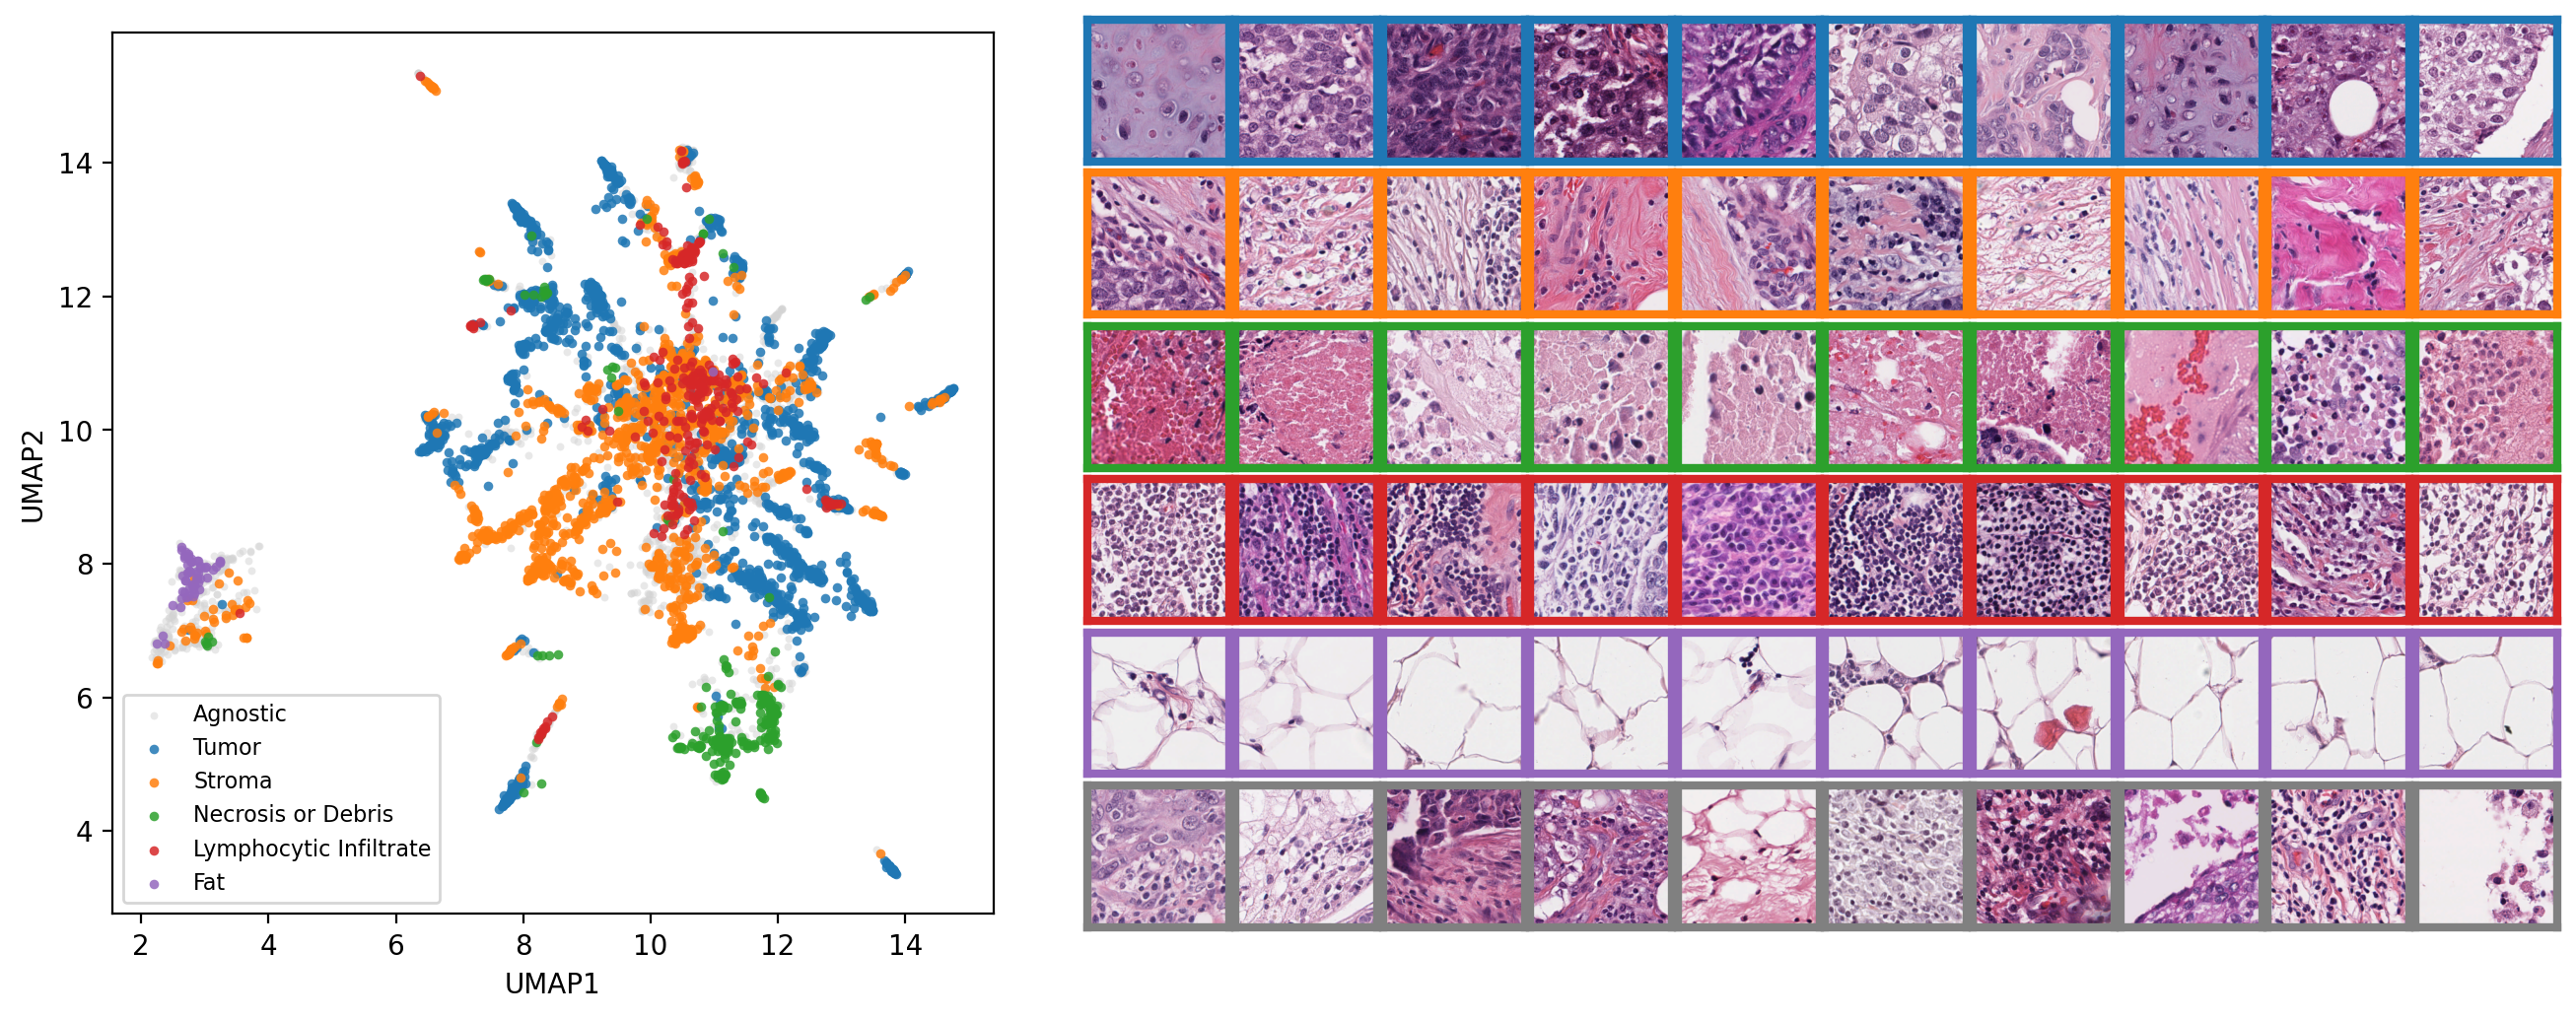
\includegraphics[width=1.0\linewidth]{images/resnet50-hematoxylin_umap_encoder_model-prediction_top-5.png}
        \end{minipage}    
    \end{subfigure}
    \begin{subfigure}{\textwidth}
        \centering
        \begin{minipage}[c]{0.05\textwidth}
            \rotatebox{90}{\textbf{JigMag}}
        \end{minipage}
        \begin{minipage}[c]{0.7\textwidth}
            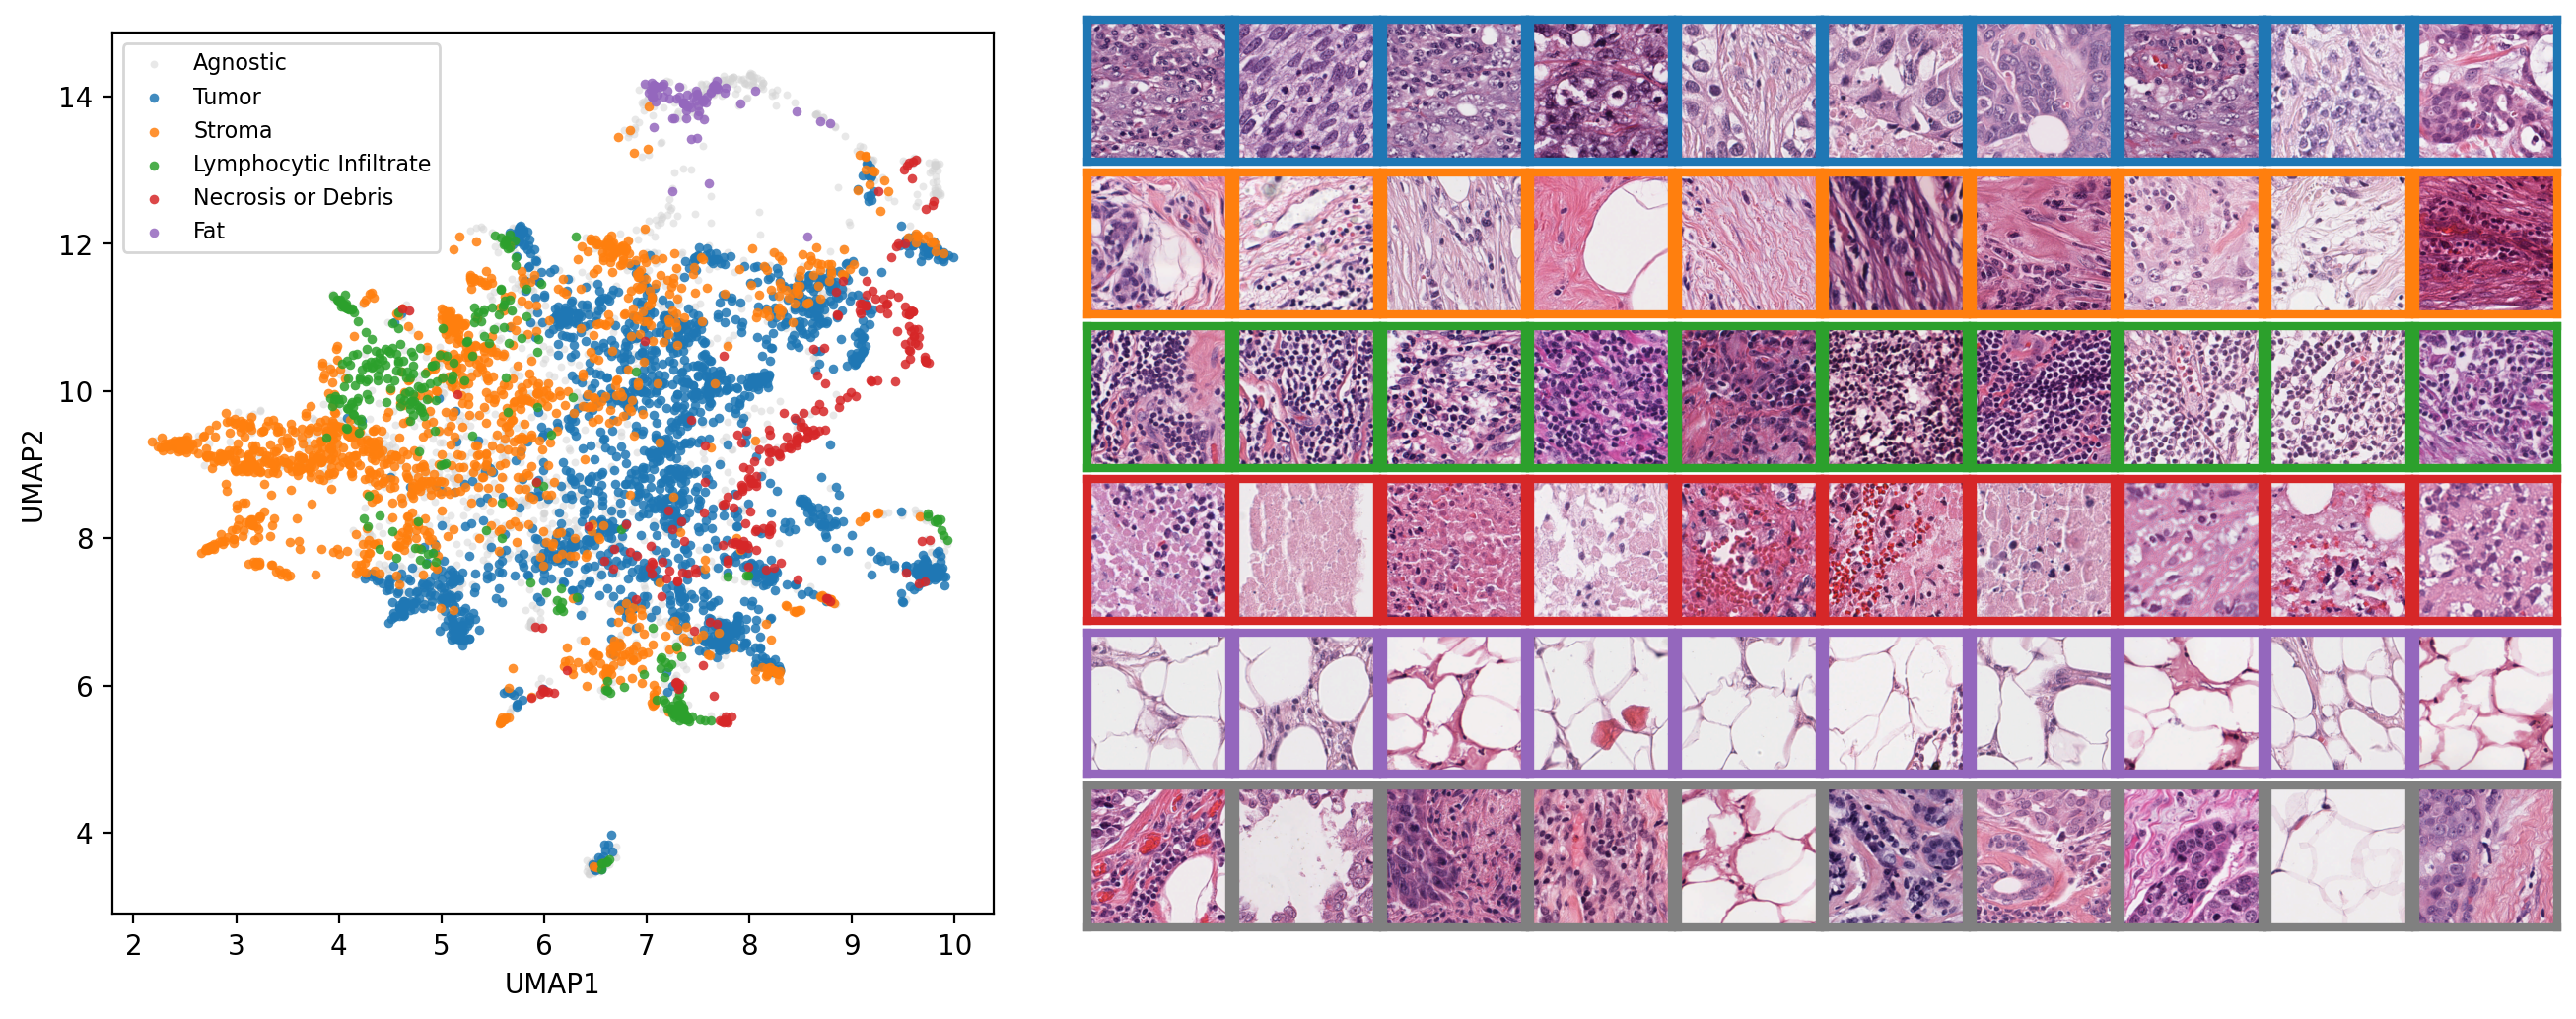
\includegraphics[width=1.0\linewidth]{images/resnet50-jigmag_umap_encoder_model-prediction_top-5.png}
        \end{minipage}    
    \end{subfigure}
    \begin{subfigure}{\textwidth}
        \centering
        \begin{minipage}[c]{0.05\textwidth}
            \rotatebox{90}{\textbf{Magnification}}
        \end{minipage}
        \begin{minipage}[c]{0.7\textwidth}
            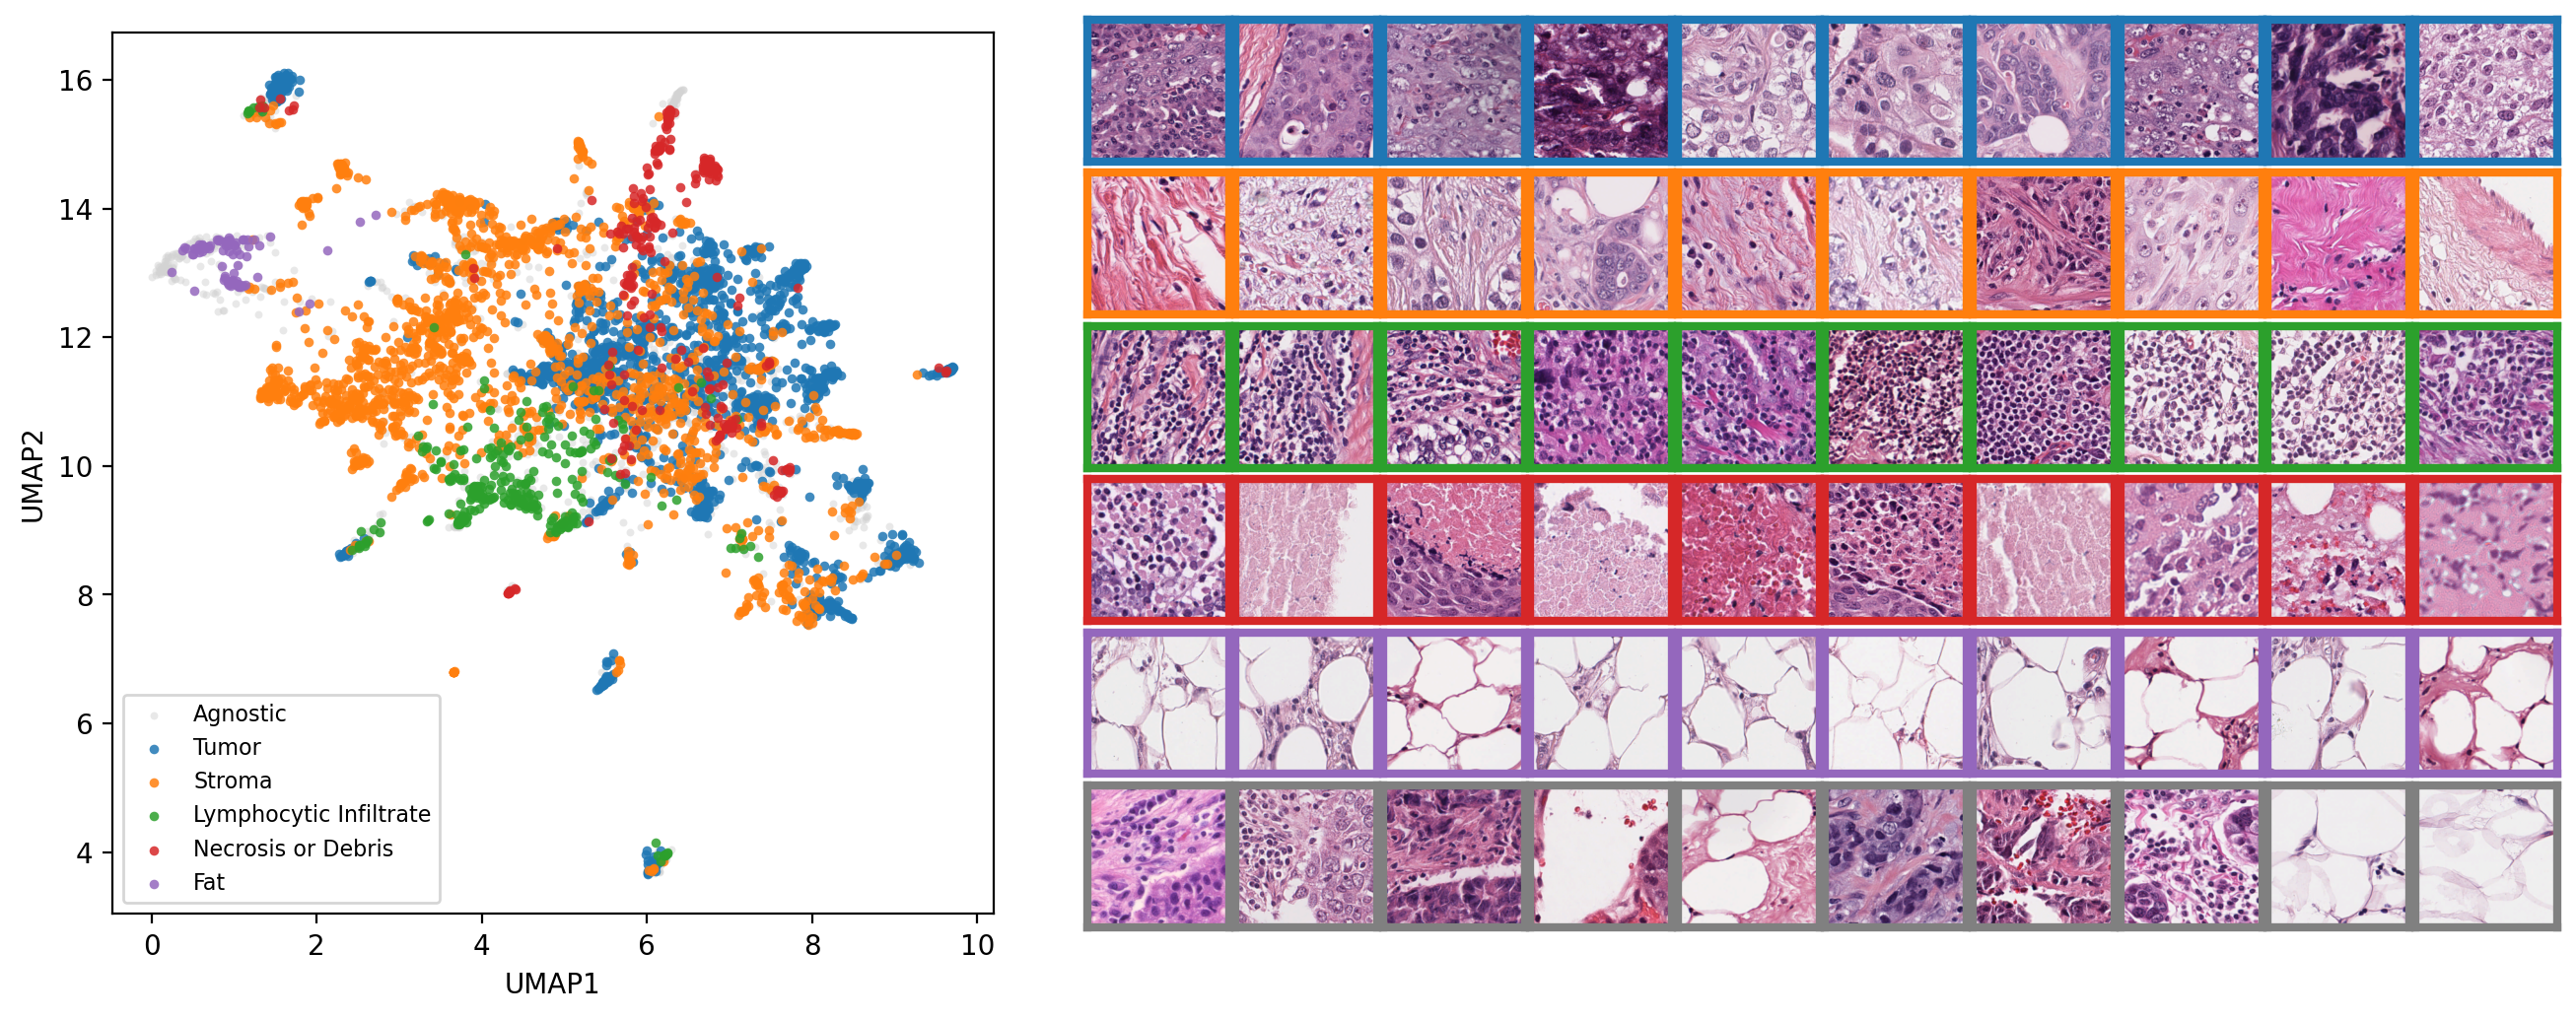
\includegraphics[width=1.0\linewidth]{images/resnet50-magnification_umap_encoder_model-prediction_top-5.png}
        \end{minipage}    
    \end{subfigure}
    \caption{\textbf{Visualization of the tile-level feature space after Stage 2.} For each pretext-task configuration, we randomly sampled 2\% of tiles from each slide in the independent test cohort and projected their 512-dimensional feature representations to two dimensions using UMAP. Each tile is shaded by its dominant tissue class, defined as the class whose proportion within the tile, as predicted by the tissue-segmentation tile encoder, is at least $p = 0.5$; tiles in which no class meets this threshold are labeled as ``Agnostic''. For clarity, we display only the five tissue classes that appear most frequently among the sampled tiles.}\label{fig:tile-featture-sapce}
\end{figure*}

\begin{figure*}
    \centering
    \begin{subfigure}{0.45\textwidth}
      
\includegraphics[width=\linewidth]{images/train_tile_learning_curves.png}
    \end{subfigure}
    \begin{subfigure}{0.45\textwidth}
        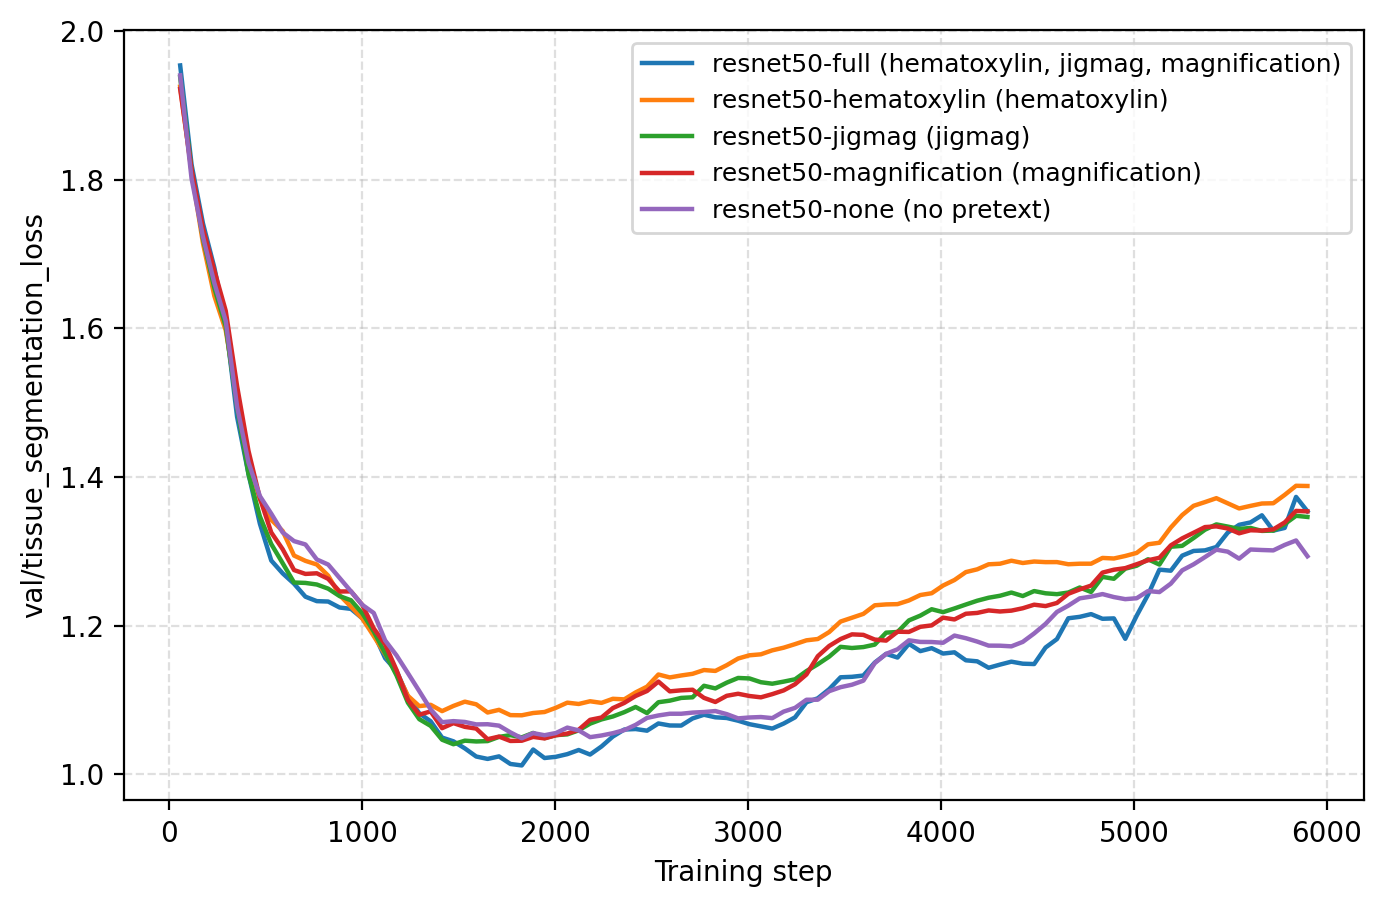
\includegraphics[width=\linewidth]{images/val_tile_learning_curves.png}
    \end{subfigure}
    \caption{\textbf{Tile-level tissue-segmentation learning curves across pretext-task configurations.} Training (left) and validation (right) tissue-segmentation loss over the course of Stage 2 training for the four pretext-task configurations: all pretext tasks combined, hematoxylin-channel prediction, JigMag, and magnification prediction. Each curve corresponds to one configuration; lower values indicate better tissue-segmentation performance.}
    \label{fig:tile-learning-curves}
\end{figure*}